\chapter{Physical and Data Link Layer:\\ Peer-to-Peer Serial Peripheral Interface}\label{sec:spi}

\section{Background}\label{sec:spi:background}

The Serial Peripheral Interface (SPI) de-facto standard is a communications protocol that is supported by almost every microcontroller in the market and a number of other embedded devices. One of the first devices to incorporate SPI was the Motorola MC68HC05C4, which was also the first device to use the name ``SPI.'' \cite{ref:1994-motorola-spi} SPI is also called ``Microwire'' in some cases, especially on older National Semiconductor devices. \cite{ref:1995-national_semiconductor-microwire}

\subsection{The SPI ``Specification''}\label{sec:spi:background:spi_specification}

SPI is a master-slave, synchronous serial communications protocol that uses either three or four wires, depending on the configuration, and typically transmits up to one fourth of the clock speed of the device. SPI is considered a ``de-facto'' standard because, although no formal specification for SPI exists, manufacturers follow the same basic protocol. A number of variations between manufacturers and chips exist, however. Unless otherwise noted, this document is referring to the typical implementation of SPI. SPI is typically intended for point to point communications, although it can also be used in a bus configuration. 

A typical SPI interface in is shown in Figure \ref{fig:spi:typical_pinout}. The Master Out, Slave In (MOSI) pin is used to transfer data from a master device to a slave device, and the Master In, Slave Out (MISO, also called SOMI) transfers data from a slave to a master. The Clock (CLK) pin clocks data on these two lines. In typical three wire implementations, MOSI, MISO, and CLK are the three pins used.

\begin{figure}[ptb]
	\begin{centering}
		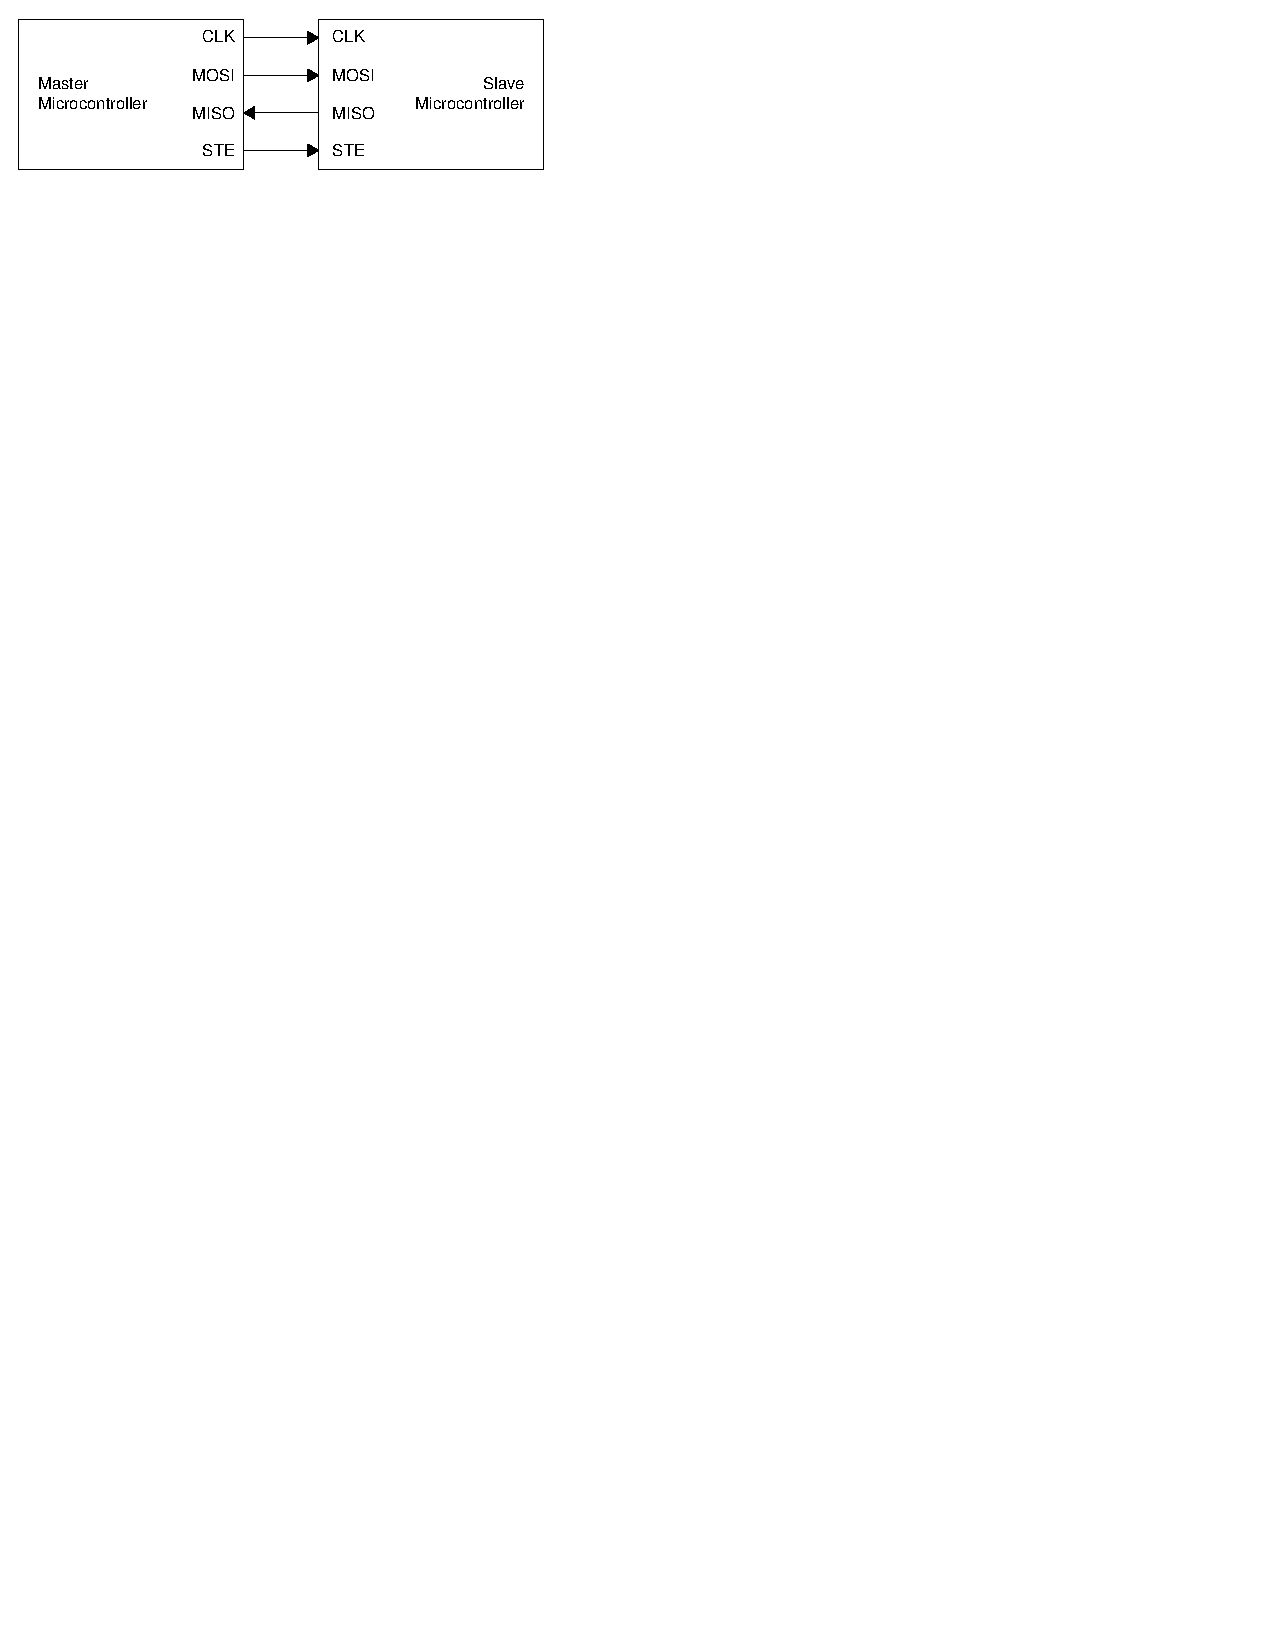
\includegraphics{SPI/Figures/spi-typical_pinout.pdf}
		\caption{Typical SPI Pinout}
		\label{fig:spi:typical_pinout}
	\end{centering}
\end{figure}

The fourth pin is the Slave Transmit Enable (STE) pin, and is where most variances between implementations occur. Typically, when asserted, the STE pin allows a slave to transmit to and receive from the master. The STE pin can be asserted high or low depending on the implementation. A variety of other configurations exist, so care must be taken to ensure that the STE pin behaves properly. For example, on the MSP430 microcontroller from Texas Instruments, the STE pin is also used to allow multiple masters on a single bus by suppressing communication from other masters, in addition to enabling slave communication \cite{ref:2009-ti-msp430}. The STE pin can also be used to allow bussed SPI transmissions. The master asserts the STE pin on the specific slave with which it wants to communicate while leaving the STE pins on the other devices de-asserted.

Typically, four clocking schemes are available to be configured. Data can be transmitted on the falling edge of the clock and received on the rising edge of the clock, or vice versa. By reading on the opposite edge of the write, the signal will have had time to settle, thus eliminating errors that would otherwise occur by reading while the signal is changing. Data can also be delayed by a half clock cycle to further increase stability. These four schemes are shown in Figure \ref{fig:spi:clocking_schemes}. Note that the master always generates the clock signal. This implies that the master must send a clock signal in order for the slave to transmit. The clock signal is generated whenever the master is transmitting, but what happens when the master has nothing to send but wants to give the slave a chance to transmit? It is customary to transmit dummy data consisting of all 0's to the slave.

\begin{figure}[ptb]
	\begin{centering}
		\subfigure[Transmit on Rising Edge, No Delay]
    {
			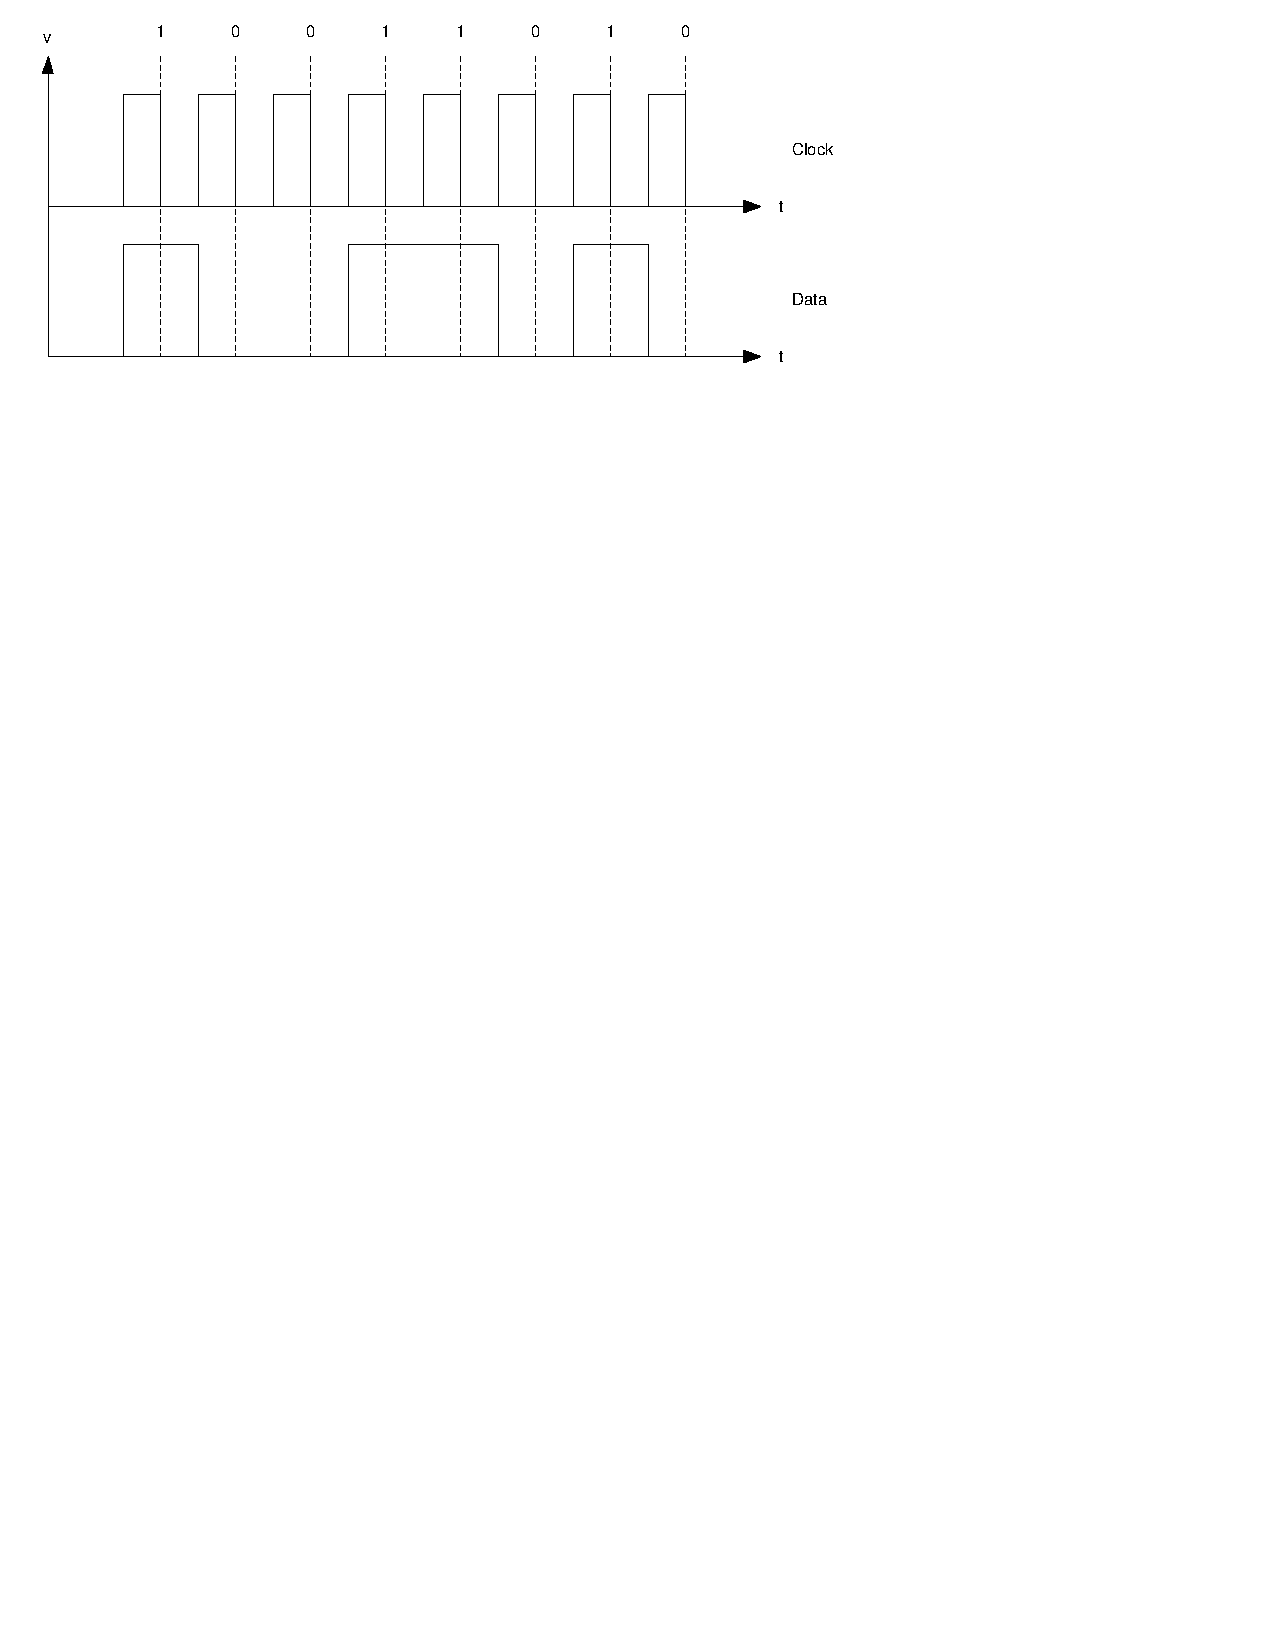
\includegraphics[width=6in]{SPI/Figures/spi-clocking_schemes_rise_no_delay.pdf}
			\label{fig:spi:clocking_schemes_rise_no_delay}
		}
		\subfigure[Transmit on Rising Edge, Half-cycle Delay]
    {
			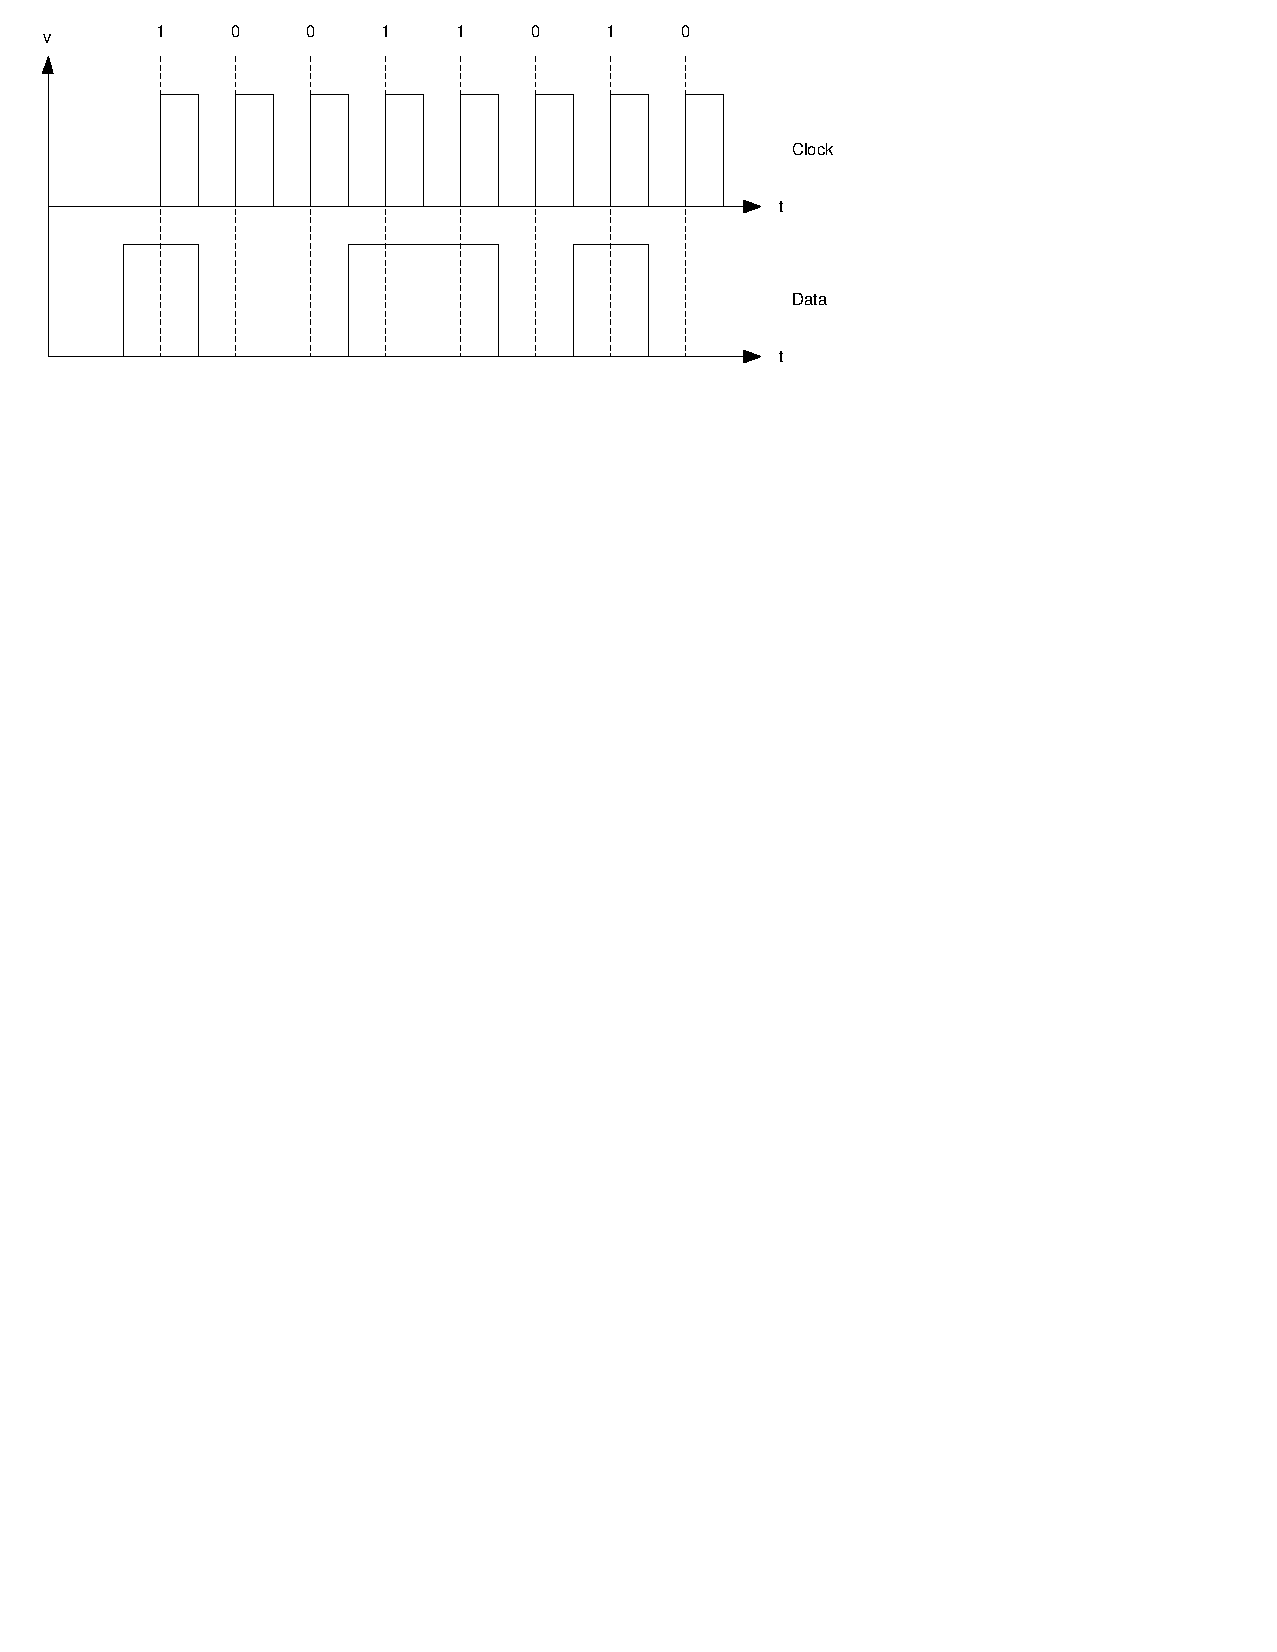
\includegraphics[width=6in]{SPI/Figures/spi-clocking_schemes_rise_delay.pdf}
			\label{fig:spi:clocking_schemes_rise_delay}
		}
		\captcont{SPI Clocking Schemes}
		\label{fig:spi:clocking_schemes}
	\end{centering}
\end{figure}

\begin{figure}[ptb]
	\begin{centering}
		\subfigure[Transmit on Falling Edge, No Delay]
    {
			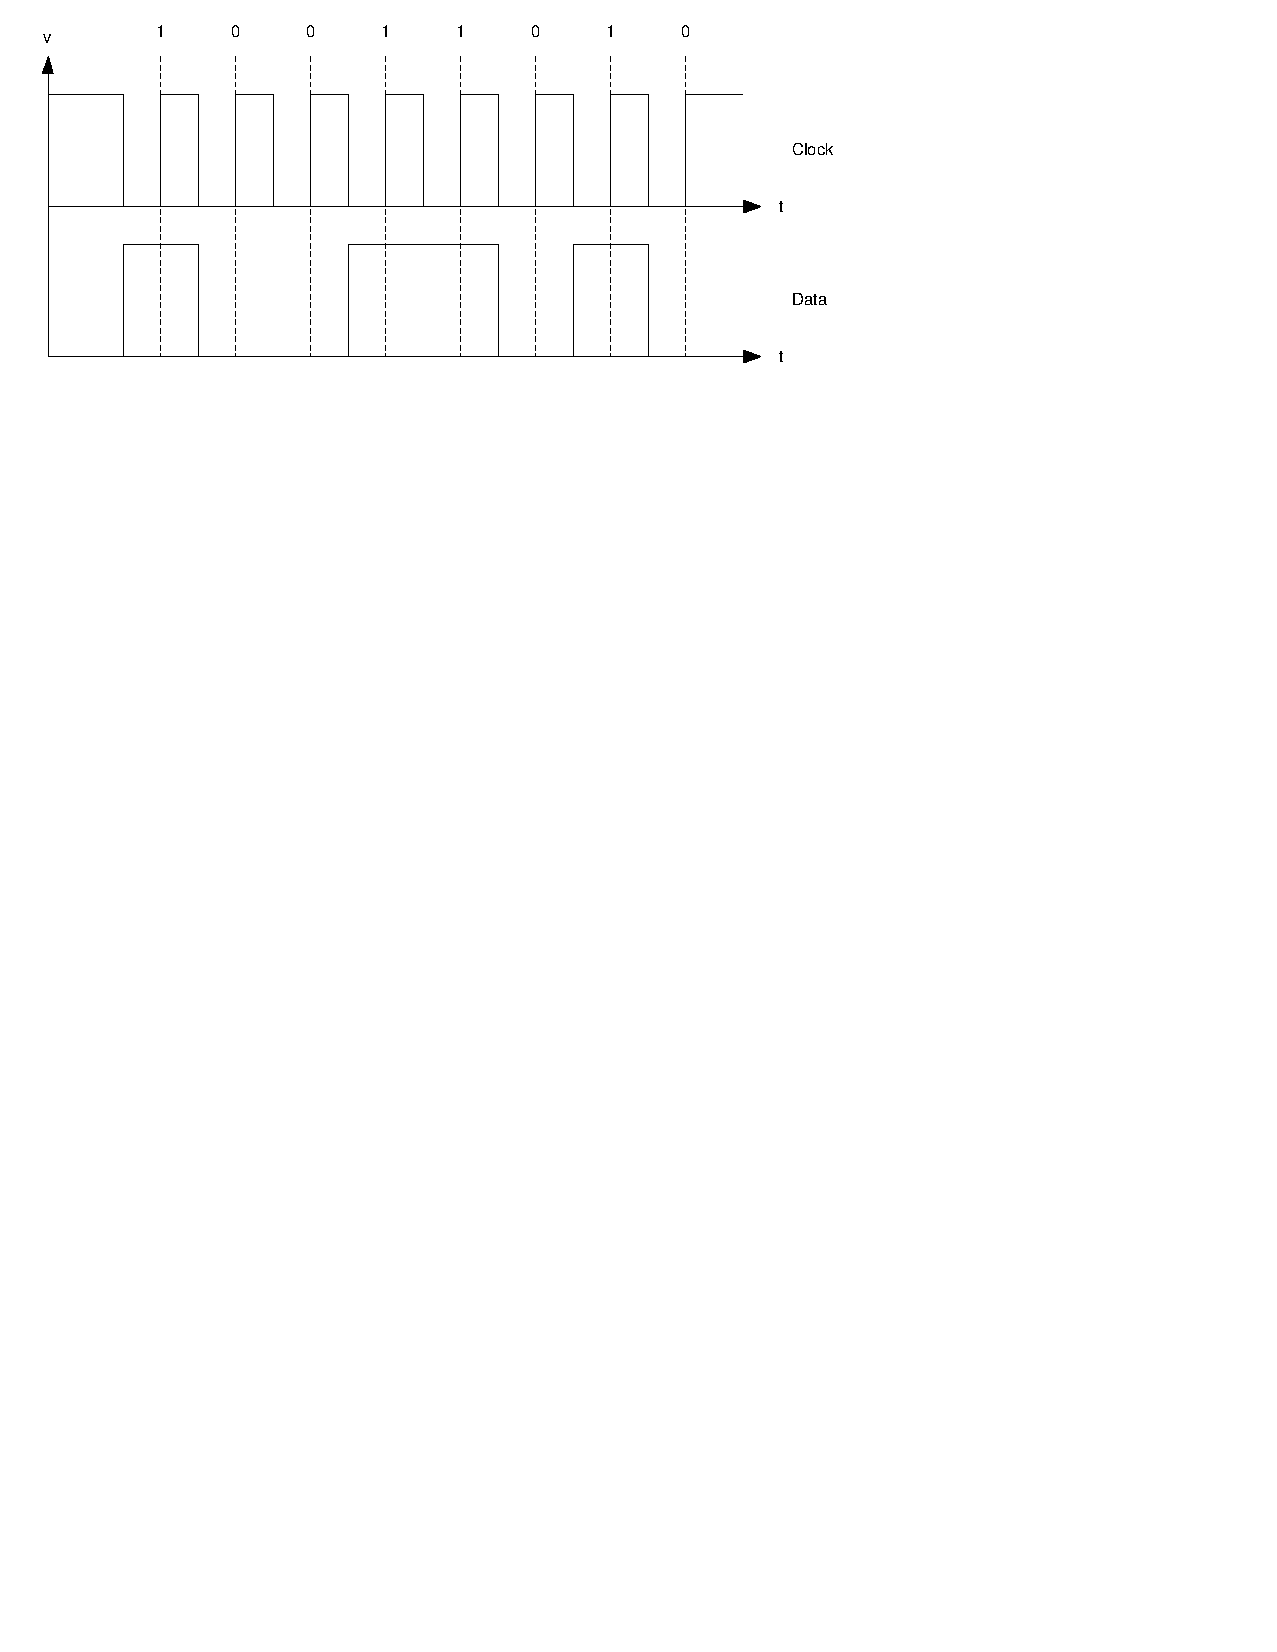
\includegraphics[width=6in]{SPI/Figures/spi-clocking_schemes_fall_no_delay.pdf}
			\label{fig:spi:clocking_schemes_fall_no_delay}
		}
		\subfigure[Transmit on Falling Edge, Half-cycle Delay]
    {
			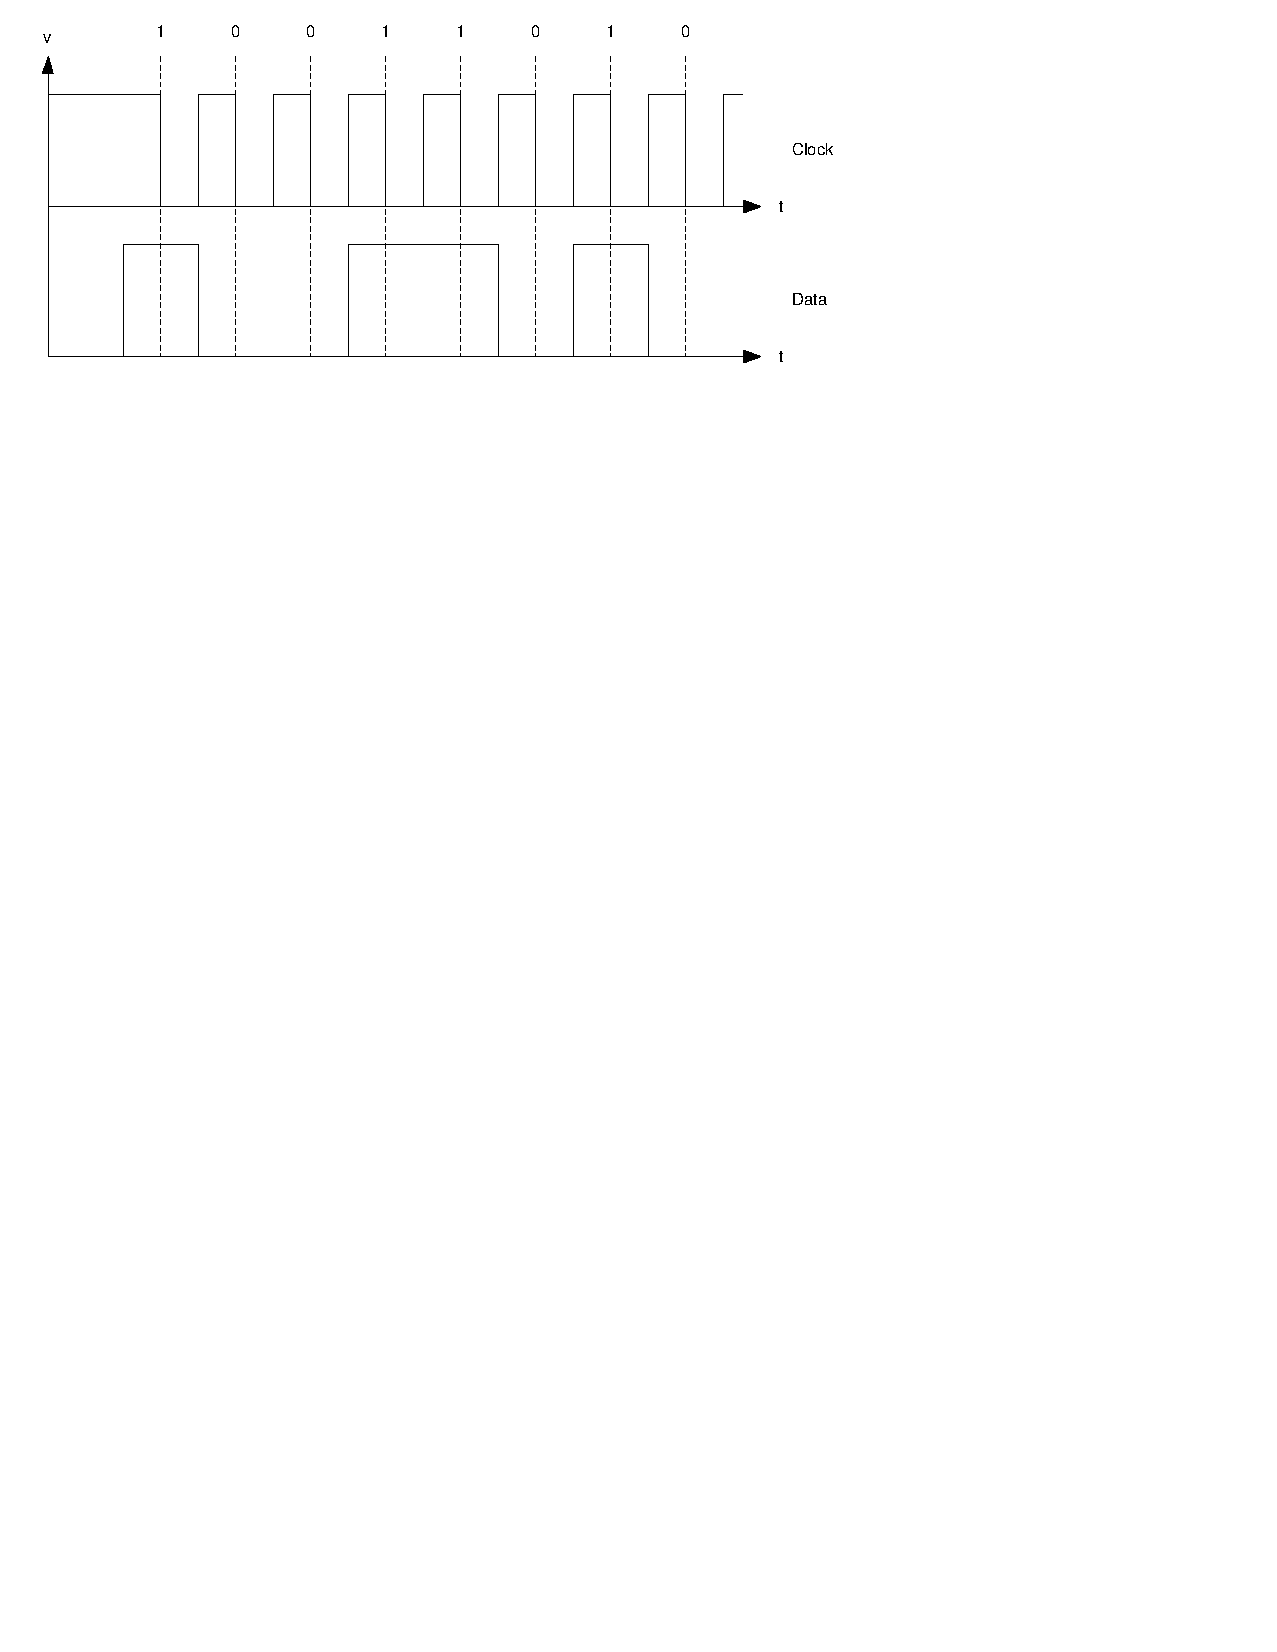
\includegraphics[width=6in]{SPI/Figures/spi-clocking_schemes_fall_delay.pdf}
			\label{fig:spi:clocking_schemes_fall_delay}
		}
		\caption{SPI Clocking Schemes cont.}
		\label{fig:spi:clocking_schemes-continue_1}
	\end{centering}
\end{figure}

\subsection{Comparison with other embedded communication protocols}\label{sec:spi:background:comparison}

Two other communication protocols are commonly found on microprocessors that are used for inter-processor communication: Inter-Integrated Circuit (), and Controller Area Network Bus (CAN-Bus).

$\textrm{I}^2 \textrm{C}$ was originally developed by Philips for use by microcontrollers in TV sets. $\textrm{I}^2 \textrm{C}$ is commonly used to connect peripheral devices such as sensors, memory, and multimedia hardware codecs to a central microcontroller. $\textrm{I}^2 \textrm{C}$ is a bus-based protocol that uses two signals: serial clock and serial data. The master controls the clock, as in SPI, to prevent devices from communicating over each other. Unlike SPI, $\textrm{I}^2 \textrm{C}$ uses a primitive packet system. Devices come with a hardwired address, with the lower bits being user-configurable. Devices only respond to a message if a packet contains the correct device address. A simple Acknowledgement (ACK) system is included in the packet protocol. Devices can communicate at three different speeds: standard devices can communicate up to 100 kbps, fast-mode devices can communicate up to 400 kbps, and high-speed-mode devices can communicate up to 3.4 Mbps. \cite{ref:2001-embedded.com-i2c} 

Because $\textrm{I}^2 \textrm{C}$ is a bussed system, the communication speed is the aggregate speed for all devices. If every controller wants to communicate at the same time, the total bandwidth in an  node system available to a fast-mode device is $\frac{400 kbps}{n - 1}$, which is considerably slower than SPI. Even in the best-case scenario of $n=2$, SPI can still run faster on devices with clock speeds in the hundreds of megahertz. Another disadvantage of bus-based systems is that the maximum size of the network is limited to a handful of nodes for all practical purposes. One advantage of $\textrm{I}^2 \textrm{C}$ is that it is an official standard, so different implementations will ``just work,'' whereas SPI can take some additional hardware to properly interface different implementations.

CAN-bus is another bus-based system that was originally developed by Bosch, an automotive parts manufacturer, as a solution to cable management problems in automobiles with a large number of microcontrollers and sensors. CAN-bus uses a two-wire differential interface carrying the data signal that can operate up to 1 Mbps. CAN-bus optionally includes ground and power lines, which allows fault-tolerance if one of the data lines is severed. CAN-bus is a peer-to-peer network that uses a clever arbitration system. The outputs of all nodes form a wired-OR network, and nodes read back everything they write to the bus to see if anyone else is also transmitting. By the time the header has been transmitted, the system has arbitrated itself without requiring re-transmission from the node that won the arbitration. CAN-bus uses a packet system that includes error detection, ACK capabilities and a data payload of 8 bytes. A few protocols are designed to run on top of CAN-bus, which further simplifies messaging. \cite{ref:2003-embedded.com-canbus}

Can-bus also suffers from the same performance issues as $\textrm{I}^2 \textrm{C}$ because it is bussed, while SPI does not suffer such issues. CAN-bus does provide a lower barrier of entry, especially when paired with a higher-level protocol, because less must be done to support messaging between nodes. CAN-bus is also a true peer-to-peer system, which is advantageous in distributed systems, as will become evident in Section \ref{sec:spi:background:distributed_systems}.

\subsection{Distributed Systems Using SPI} \label{sec:spi:background:distributed_systems}

Before SPI can be used effectively as the underlying protocol for a distributed system, one concern must be addressed: SPI is a master/slave protocol. While it is possible to realize a distributed system with SPI's master/slave system, it would be extremely difficult. For example, if three nodes are connected to each other in a ring, then which nodes should be masters and which nodes should be slaves? There isn't a solution in this case, and there are many other topologies that can't be realized in a master/slave situation if the node is configured fully as a master or fully as a slave. Mixed configurations, a.k.a. one port is a master and the other is a slave, can solve this problem, but it adds complexity for the end-user. In the topologies that can be implemented with a master/slave system, the issue remains of configuring each node manually to be a master or a slave. The other problem is one of utilization. In order for a slave to transmit, the master must also transmit, which can be inefficient because the master does not know when the slave wants to transmit. If the master does not transmit all the time, then a delay is incurred when the slave wants to transmit but must wait for the master to transmit. One solution to this problem is for the master to transmit dummy data all the time, but aside from inelegance, the problem of determining which data is dummy data and which data is valid data must be solved. These are solvable problems, but they require more complex code and overhead. A peer-to-peer system is the preferred method to provide a true plug-and-play system that is easy for the user to implement and is efficient. 

\section{Objectives}\label{sec:spi:objectives}

As mentioned in Chapter \ref{sec:introduction}, the physical and data link layer must meet the following criteria: 
\begin{enumerate}
	\item Scalable
	\item Available on a wide variety of devices
	\item Peer-to-peer
\end{enumerate}

\section{Methodology}\label{sec:spi:methodology}

As discussed in Section \ref{sec:spi:background:comparison}, bussed systems are not scalable and do not satisfy the scalability objective. SPI is a suitable choice for use in a distributed system with multiple processors, as long as it is used as a point-to-point protocol and not as a bussed protocol, which satisfies the first two objectives. An example of the suitability of SPI to distributed systems can be found in \cite{ref:2007-szekacs-multiprocessor_spi_system}, where the authors began their project using $\textrm{I}^2 \textrm{C}$  but soon ran into limitations and expanded it using SPI.

In order to satisfy the third objective, the question becomes: how does one change SPI into a peer-to-peer protocol? Looking back at figure \ref{fig:spi:typical_pinout}, notice that the same lines are used for both slave and master configurations, and that the only difference between a master and a slave is the software configuration. This makes it possible to switch a device from a slave to a master and back dynamically. Changing a processor from a slave to a master and back forms the crux of the proposed solution.

In the solution, every device is configured as a slave by default. Whenever a device must communicate with a neighbor, it temporarily changes \emph{only the port connected to the neighbor} to a master. This gives a proper master/slave configuration on that port, while allowing the other ports to arbitrate to whatever configuration is required for that link. This process is called ``port elevation.'' Once elevated, the node transmits one flit\footnote{A flit is the basic unit of data in a transmission, similar to a Minimum Addressable Data Unit (MADU) in memory} of data. When the transmission is complete, the node reverts back to a slave, called ``port demotion.'' Two problems exist with this mechanism. The first problem is that this reduces SPI to a half-duplex transmission mechanism, but this issue is deemed as an acceptable loss because the bandwidth left is still much greater than that of the other mechanisms. The second problem is that no mechanisms are in place to prevent transmission collisions.

To prevent collisions, an arbitration scheme has been developed that uses the MISO pin as a GPIO pin, called the Master Arbitrate (MARB) pin. This connection is illustrated in Figure \ref{fig:spi:p2p_pinout}. The arbitration process is shown in Figure \ref{fig:spi:arbitration_scheme} and guarantees that a node will not transmit over another node. The arbitration scheme works by first checking the MARB line to see if another node is transmitting. If not, then the port attempts to claim the line by asserting MARB. Two nodes could attempt to talk at the exact same time, which would go unnoticed, so the node then waits for a pre-determined period of time that is different than the other node, and then checks the MARB line again to see if the other node has attempted to elevate. This mechanism guarantees against collisions because each node is forced to wait a different amount of time before checking again. The wait time is assigned based on the port number, which guarantees different wait times as long as the same two port numbers are not connected.

\begin{figure}[ptb]
	\begin{centering}
		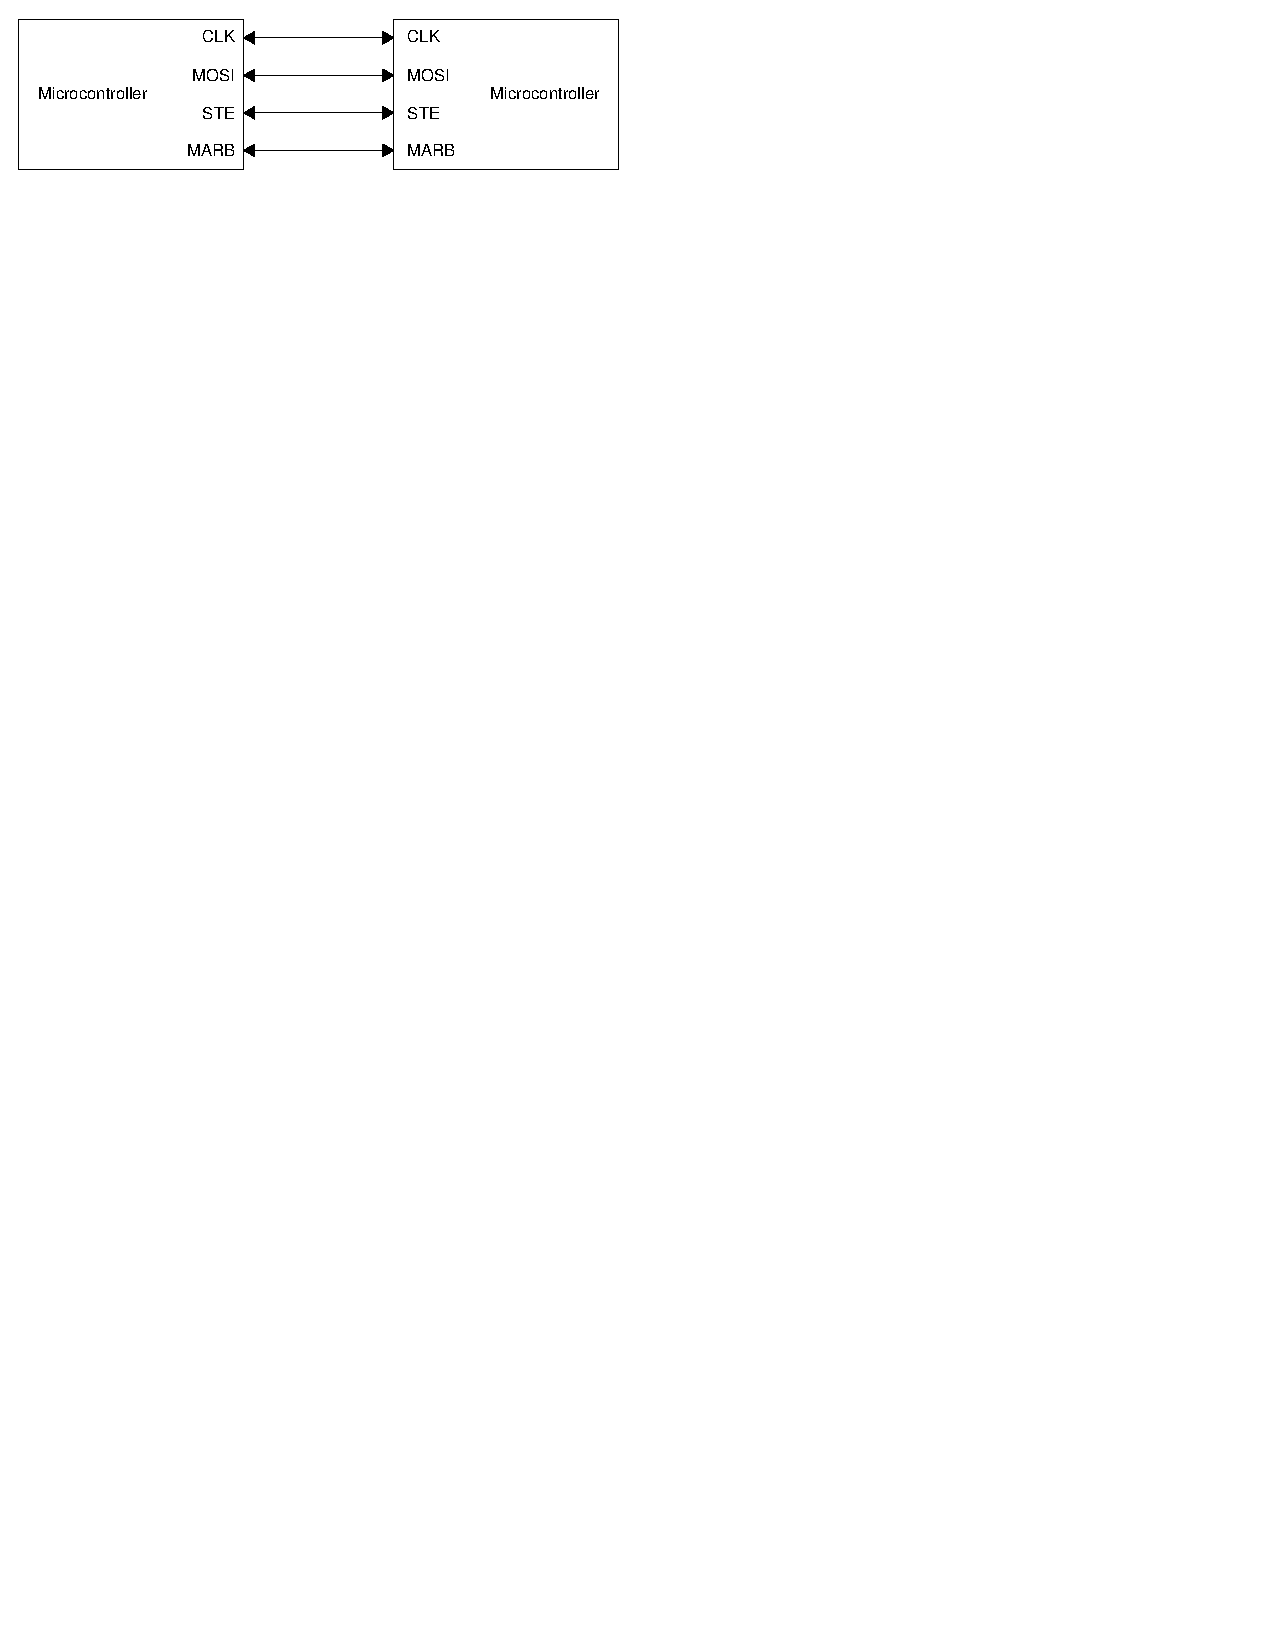
\includegraphics{SPI/Figures/spi-p2p_pinout.pdf}
		\caption{Pin-out for Peer-to-Peer based SPI}
		\label{fig:spi:p2p_pinout}
	\end{centering}
\end{figure}

\begin{figure}[ptb]
	\begin{centering}
		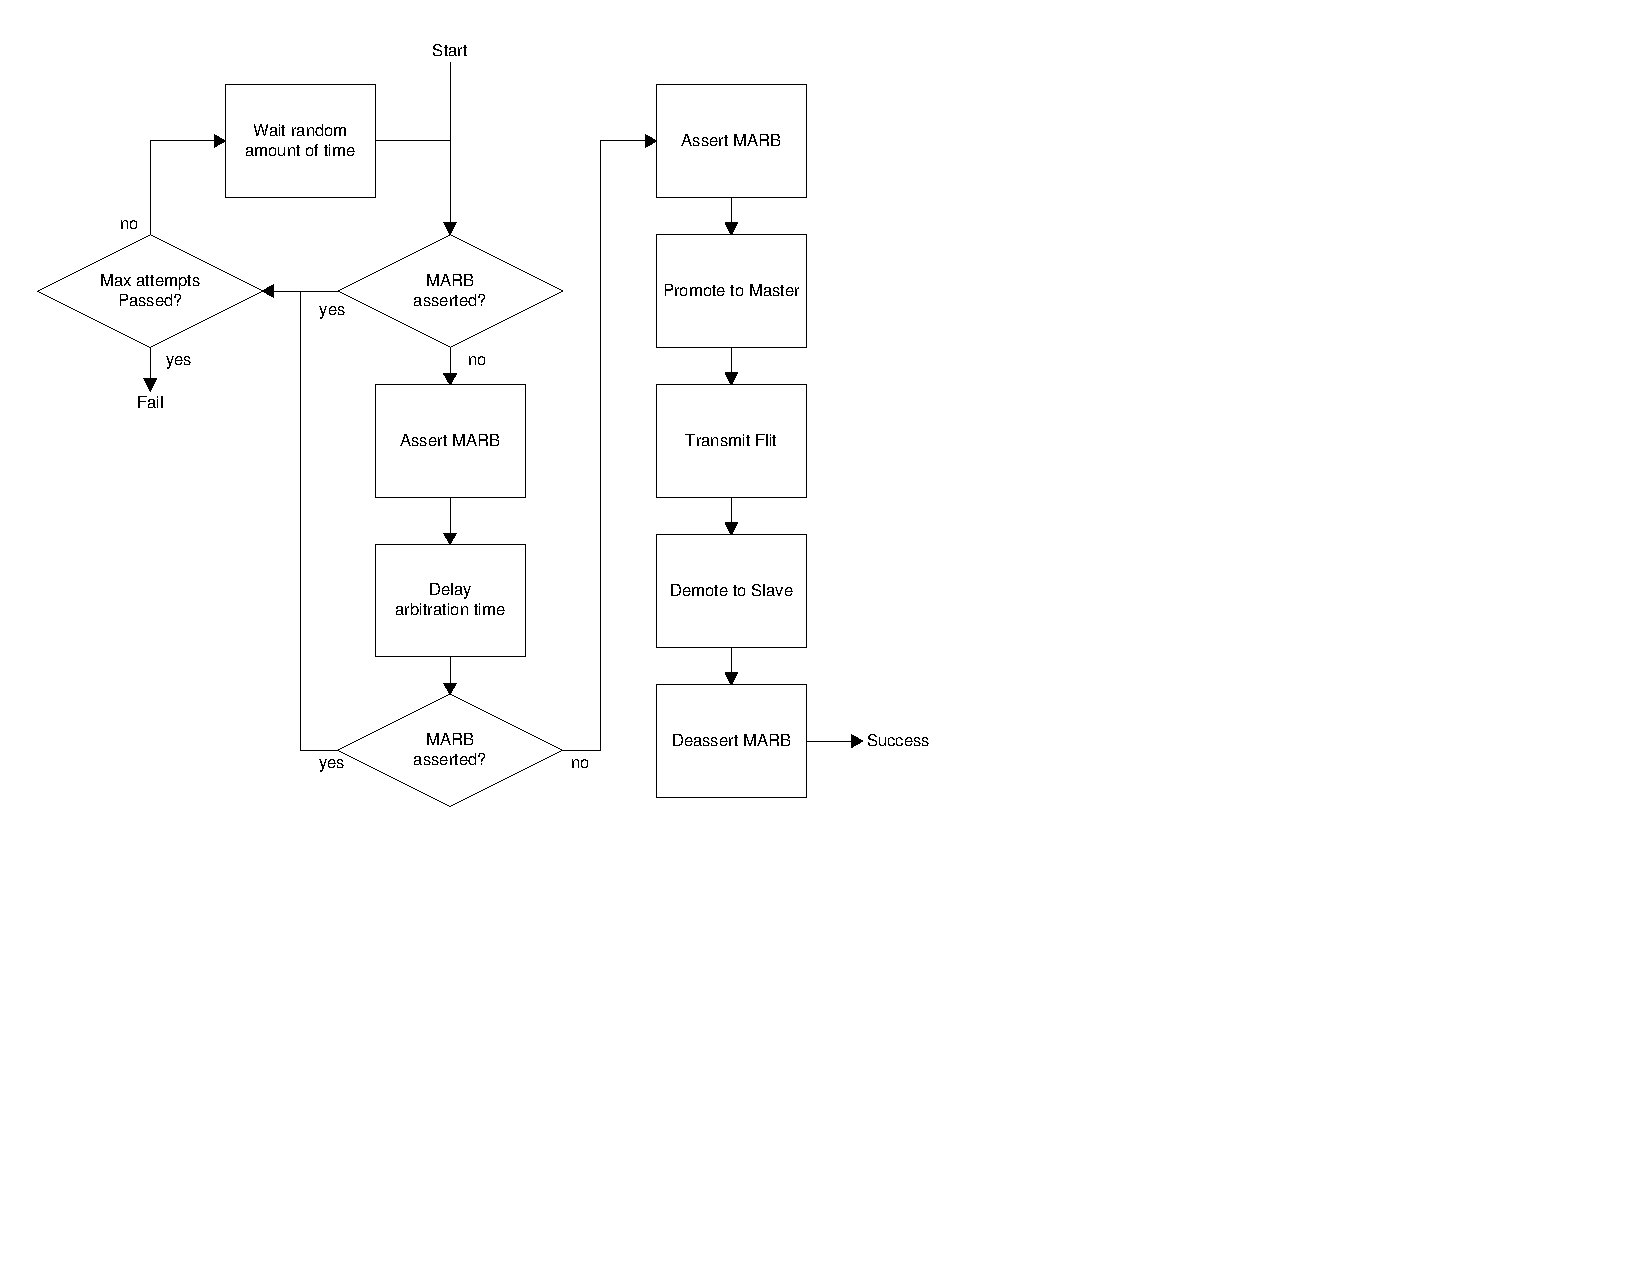
\includegraphics{SPI/Figures/spi-arbitration_scheme.pdf}
		\caption{Arbitration Scheme}
		\label{fig:spi:arbitration_scheme}
	\end{centering}
\end{figure}

To improve performance of the system, virtual channels are employed. A virtual channel is a logical channel that resides on top of a physical channel. Multiple virtual channels can be used on a single physical channel as long as each flit has a means of identifying the virtual channel on which it resides. Using multiple virtual channels allows the transmitter to interleave flits from different packets, which improves performance. In systems that do not use virtual channels, a large packet sent across a physical channel prevents smaller packets from using that channel, which increases latency and can potentially cause buffer overflows. If virtual channels are implemented, however, the smaller packets can be sent in parallel with the large packet, which eliminates that bottleneck.\footnote{For more information on Virtual Channels, read chapter 2 section 4 of \cite{ref:1997-duato-interconnection_networks}}
Determining how many virtual channels to use is very important, especially if the base flit size is small. If too few virtual channels are used, then channels can still become blocked by transmissions. If too many virtual channels are used, then the overhead necessary to identify which virtual channel a flit is on can become proportional to the flit itself. Through experimentation, 16 virtual channels (4 bits of overhead) are enough to eliminate bottlenecks the majority of the time while keeping overhead low in this application. 
Each flit is 144 bits long. 128 bits are reserved for the network layer, and the remaining 16 bits are used for the Data Link Layer, shown in Figure \ref{fig:spi:data_link_header}. The header contains the destination address of the flit, the virtual channel on which the flit is being transmitted, and the flit type. The destination address isn't really a data link layer function, and is more or less included as padding to make the flit size a multiple of 16 and to make obtaining the destination address during processing easier. The flit type field is used to identify which of the possible flit types, shown in Table \ref{tab:spi:flit_types}, this flit is. The flit type lets the network-level protocol stack know what to do with the flit. The virtual channel field indicates the virtual channel on which this flit is being transmitted. Virtual channel 0 is reserved for system use, virtual channels 1-14 are for data transfers, and virtual channel 15 is for network-level packet headers. Headers are given a dedicated virtual channel because a) headers occupy a single flit and thus don't require virtual channels to be reserved and b) a dedicated channel ensures that packet headers can always flow through the system unimpeded.

\begin{figure}[ptb]
	\begin{centering}
		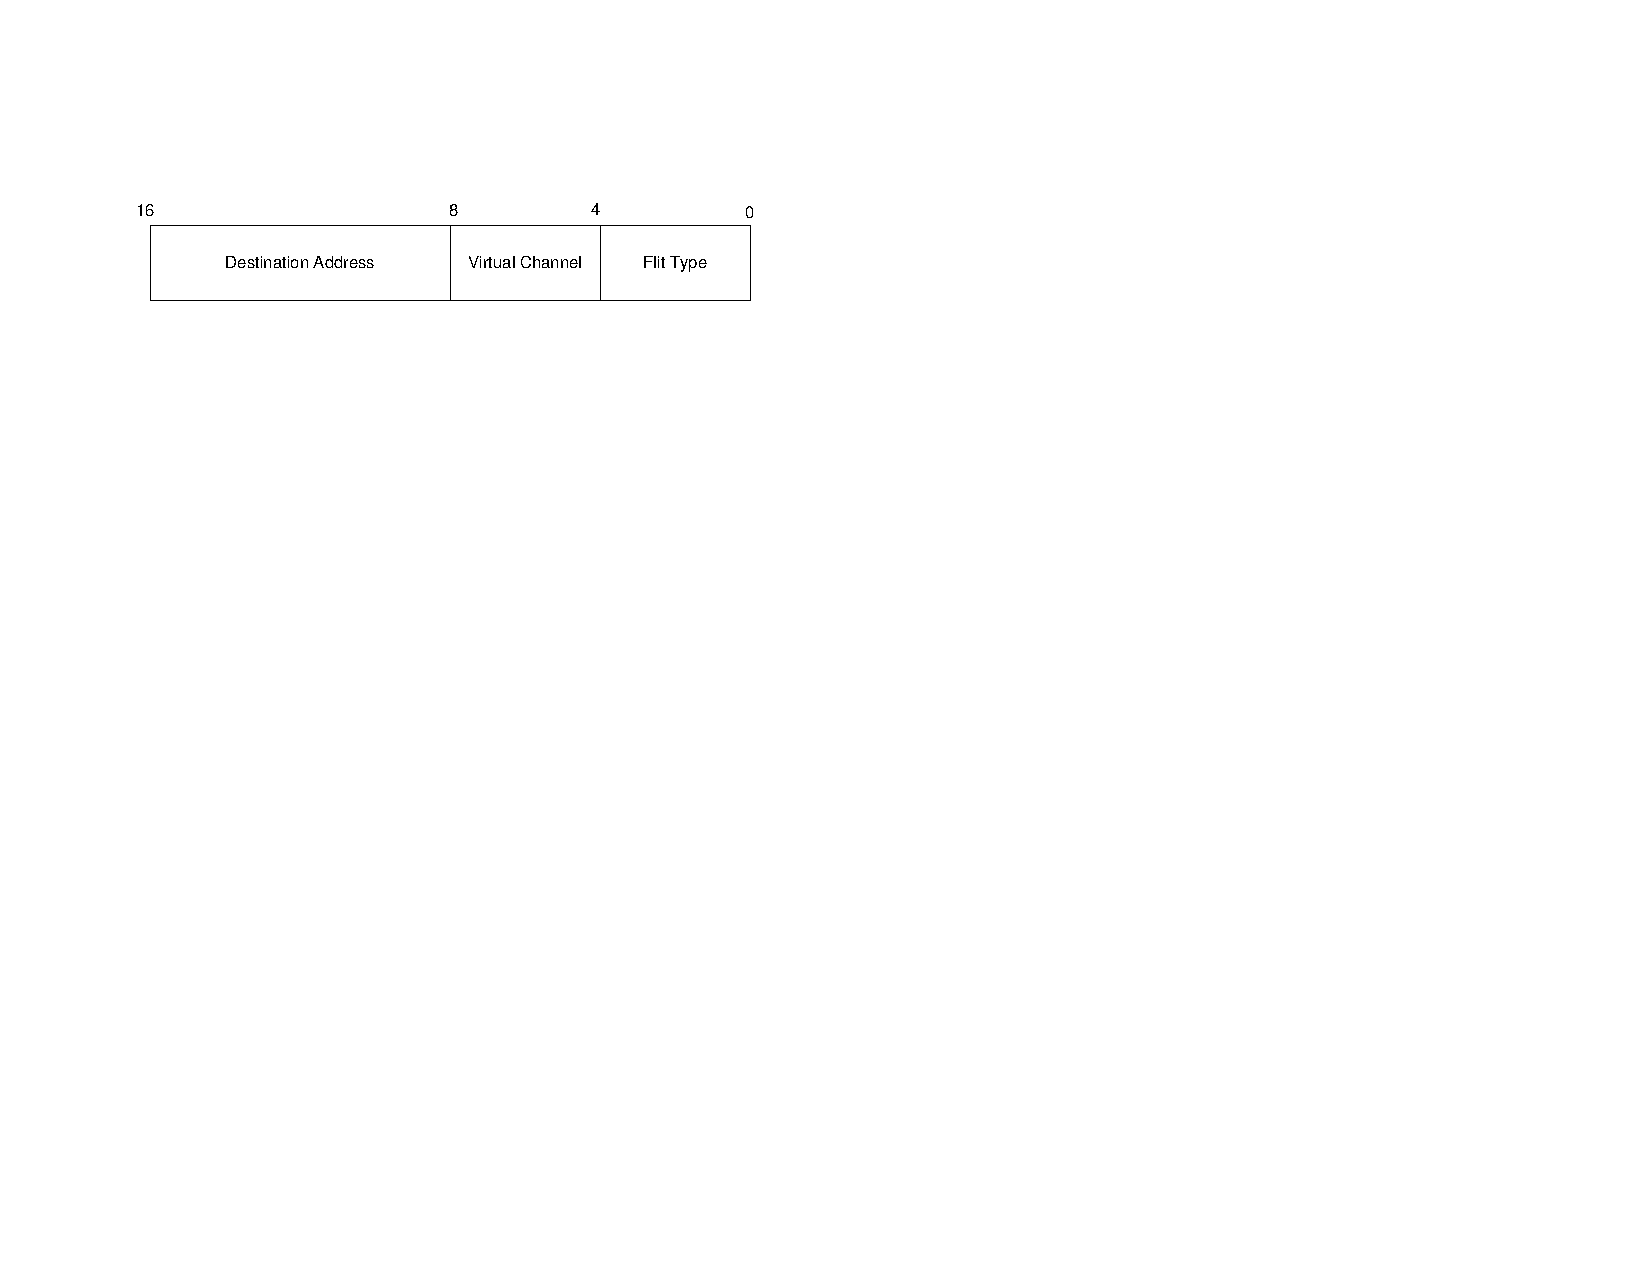
\includegraphics{SPI/Figures/spi-data_link_header.pdf}
		\caption{Data Link Layer Header}
		\label{fig:spi:data_link_header}
	\end{centering}
\end{figure}

\begin{table}
	\begin{center}
	\setlength{\extrarowheight}{1.5pt}
		\caption{List of Flit Types}
		\vspace{0.1cm}
		\begin{tabular}{|l|l|}
			\hline
			\textbf{Flit Type} & \textbf{Description}	\\
			\hline
			\hline
			Header	& A protocol-level header packet \\
			\hline
	       Payload	& Part of a protocol-level data payload \\
			\hline
	       End of payload	& Last flit in a protocol-level data payload \\
			\hline
		\end{tabular}
		\label{tab:spi:flit_types}
	\end{center}
\end{table}

In traditional implementations, each virtual channel gets its own receive and transmit buffers. If buffer capacity can be easily extended to provide each virtual channel with the same buffer capacity that a single physical channel would otherwise have, then this configuration is no problem. However, this method isn't feasible in systems with limited memory. In order to give each virtual channel its own buffer in this environment means shrinking the size of the buffers. Instead, a more efficient approach is used whereby a single receive buffer is shared by all virtual channels across all ports, and one shared transmit buffer is shared by all virtual channels for each port. Buffers are shared across virtual channels because only some of the virtual channels will be used at any specific point of time. If buffers were not shared, then the input buffer for one virtual channel could overflow, while the others remained empty. A single input buffer is used across all ports because the port which a flit arrives usually has little, if any, impact on where it is going.

\section{Implementation}\label{sec:spi:implementation}

The software implementation for the physical and data link layers are divided into three groups: buffer management, transmission, and reception.

\subsection{Buffer Management Functions}\label{sec:spi:implementation:buffer_management_functions}

Three functions are used to enqueue and dequeue flits from the buffers: \lstinline$EnqueInboundFlit()$, \lstinline$DequeInboundFlit()$, and \lstinline$EnqueOutboundFlit()$. Dequeueing of outbound flits is handled directly by the transmission software for performance reasons, and thus there is no separate function for it. The buffers are implemented as circular buffers; they are declared as static arrays and a pointer to the head and tail of the queue keeps track of the queue. This makes it very efficient to enqueue/dequeue an item because other items do not need to be shifted around after an item is added/removed. 

Each buffer has a control function associated with it that runs in its own thread. \lstinline$ProcessInboundFlits()$, described in Section \ref{sec:spi:implementation:reception}, dequeues flits from the receive buffer and processes them. \lstinline$ProcessOutboundFlits()$, described in Section \ref{sec:spi:implementation:transmission}, dequeues flits from the transmit buffer and transmits them on the appropriate port. These threads and their relationships to the buffers are illustrated in Figure \ref{fig:spi:software_architecture}. These functions drive the rest of the system in a data-driven manner.

\begin{landscape}
	\begin{figure}[ptb]
		\begin{centering}
			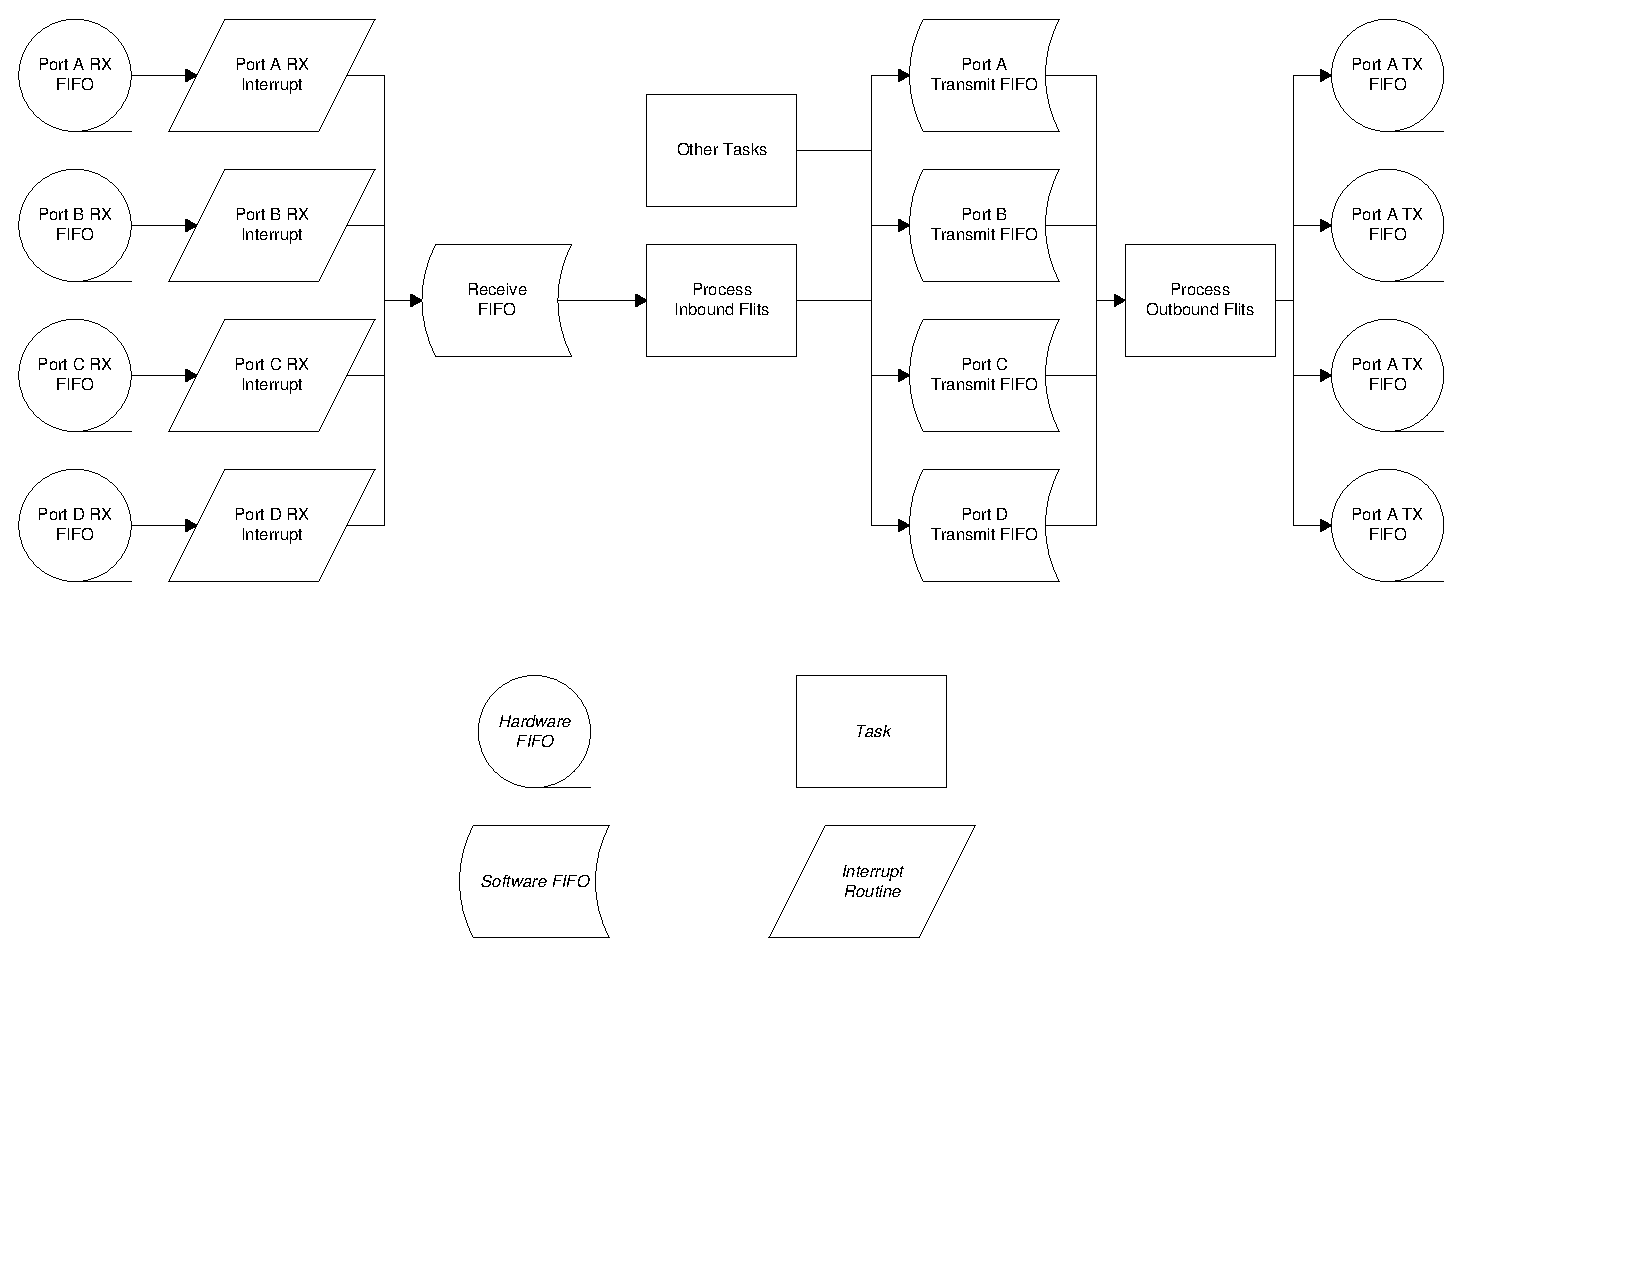
\includegraphics[width=8.5in]{SPI/Figures/spi-software_architecture.pdf}
			\caption{Software architecture of SPI systems}
			\label{fig:spi:software_architecture}
		\end{centering}
	\end{figure}
\end{landscape}

\subsection{SPI Transmission}\label{sec:spi:implementation:transmission}

Each port is configured to run at 20 MHz because the time spent in this function must be minimized, and this speed was experimentally found to be the fastest reliable speed which the F2808 can run. The SPI is configured to use 16-bit words. It makes sense to configure the SPI FIFOs to contain a single flit, so the receive FIFO is configured to interrupt when 9 words (144 bits) have been received. The SPI is configured to transmit on the falling edge of the clock, without a delay. This configuration was chosen because it is the most common configuration among SPI devices.

There is a single transmission function: \lstinline$ProcessOutboundFlits()$. This code is extremely sensitive to timing, and so interrupts are disabled when this function is running. In addition, this thread has the highest priority of all running threads, which prevents any other threads from running. To prevent the rest of the system from being locked, this function must be as efficient as possible. The function is implemented as a state diagram with five possible states plus an error state. This function must manage all ports on the device simultaneously, and many of these states require a delay between them. Using states allows the function to interleave the transmission for each port. The code works by checking whether each port is in a given state in the order shown in Figure \ref{fig:spi:transmit_state_charts}, and if so, executes according to the associated flow-chart. This has the effect of causing the ports to run in ``lock-step'' with each other in most cases, although each port does have the freedom to diverge in the case of arbitration issues. 

\begin{landscape}
	\begin{figure}[p]
		\begin{centering}
			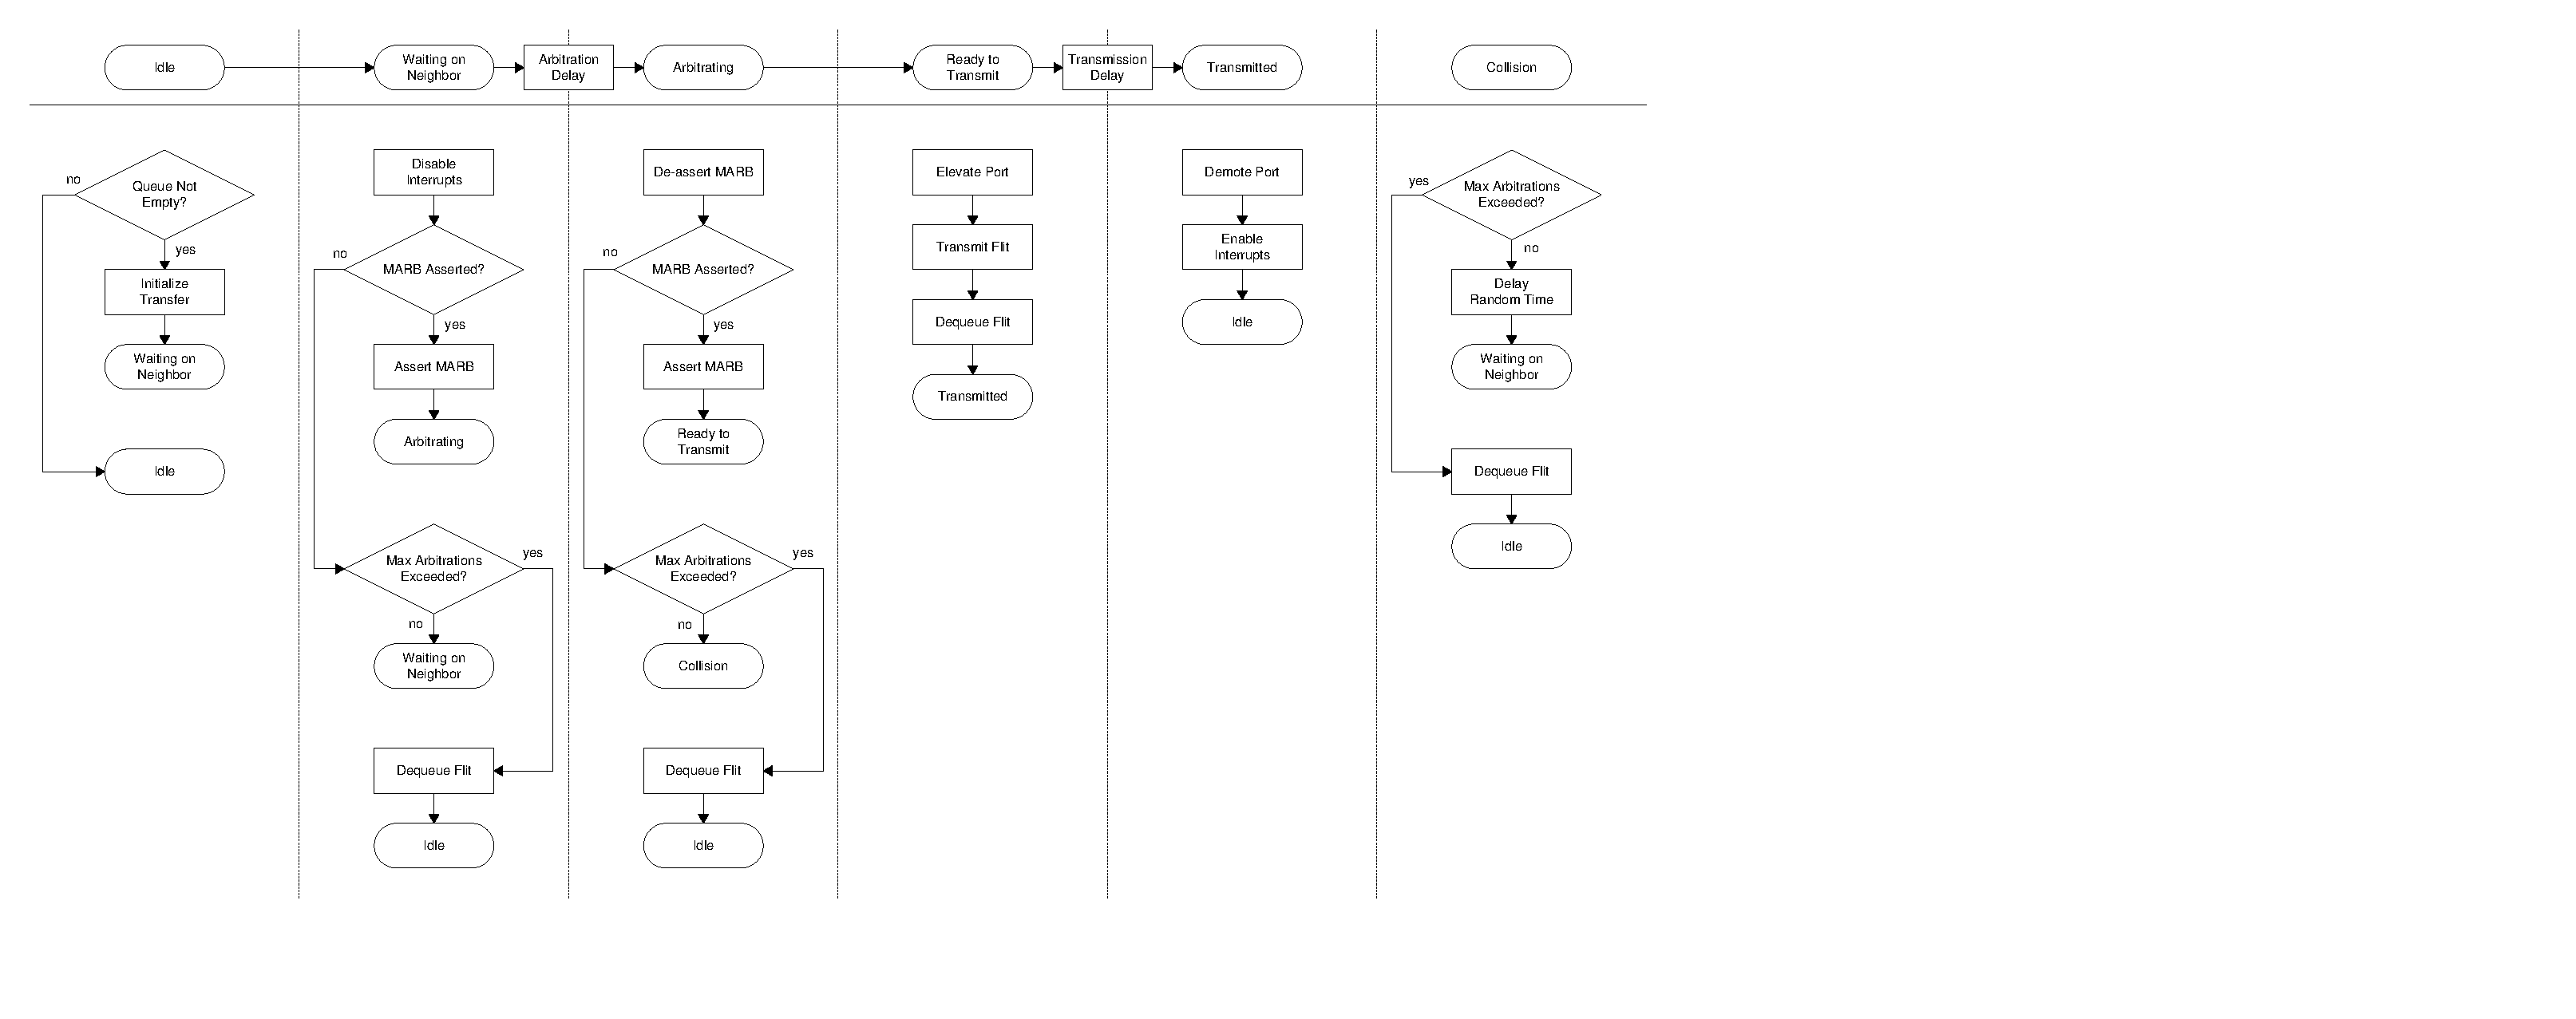
\includegraphics[width=8.5in]{SPI/Figures/spi-transmit_state_charts.pdf}
			\caption{Flowchart of States for \lstinline$ProcessOutboundFlits()$}
			\label{fig:spi:transmit_state_charts}
		\end{centering}
	\end{figure}
\end{landscape}

One interesting side-effect of the port elevation and demotion was uncovered during the development process: all of the internal logic on the F2808 is hardwired for input or output, regardless of whether or not the port is a master or slave. The upshot of is that the interrupt logic for the receiver in slave mode becomes the interrupt logic for the transmitter in master mode. As a result, this caused the F2808 to trigger a receive interrupt after a port was demoted and thus called the receiver interrupt routine, even though no data had actually been received! The solution is to reset all interrupts after the port has finished transmitting but before the port is demoted, and the interrupt is squashed before it reaches the PIE.

\subsection{SPI Reception}\label{sec:spi:implementation:reception}

SPI reception is composed of two primary parts: the SPI interrupt and the \lstinline$ProcessInboundFlits()$ function. The interrupt routine dequeues the flit out of the SPI FIFO, enqueues the flit in the inbound flits queue, and wakes up the \lstinline$ProcessInboundFlits()$ function if need be. The \lstinline$ProcessInboundFlits()$ function first dequeues the oldest flit in the inbound flits queue. If the flit is a header flit, it is sent on to be processed by the network-level protocol stack, described in Chapter \ref{sec:protocol}. If the flit is a data payload flit, then it directly enqueued into the appropriate outbound flit queue. If the flit is the end of a data payload, it is enqueued into the appropriate outbound flit queue, and the stored transmission information is finalized. Note that the protocol stack handles setting up the transmission information. Moving the major flit processing out of the interrupt routine and into a separate thread keeps the interrupt routine really short and prevents it from blocking other threads for too long. In the event that the receive buffer is full after a flit has been enqueued, then all MARB pins are asserted as a flow control mechanism to prevent any other nodes from transmitting until a flit is dequeued from the buffer.

\section{Results}\label{sec:spi:results}

To ensure that the links behaved as expected, the lines were inspected electrically to examine the waveforms. Figure \ref{fig:spi:link_waveform} shows the relevant signals for a single link. Figure \ref{fig:spi:waveform_comparison} shows the MARB signals across the four links. Note that when the MARB signal goes low, it is checking the other signal to see if there was a collision. There is no possibility of missing a collision because each link checks at a different time, unless the same links are connected together, which is an easily avoidable configuration.

\begin{landscape}
	\begin{figure}[p]
		\begin{centering}
			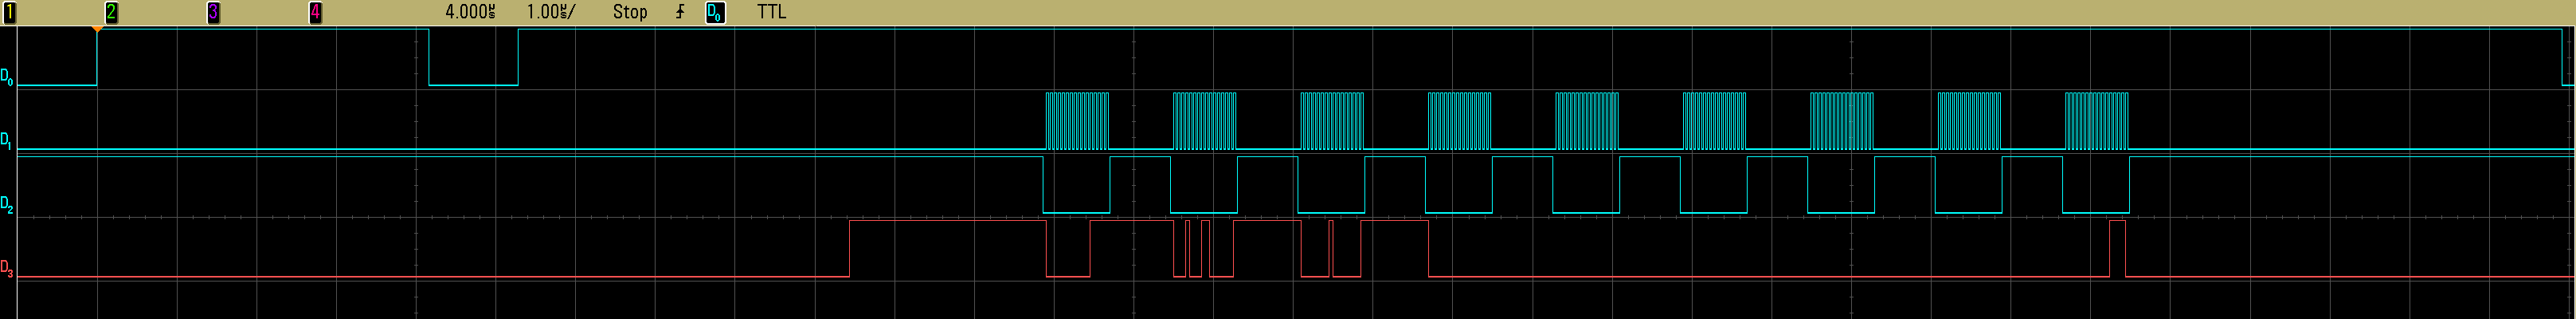
\includegraphics[width=8.5in]{SPI/Figures/spi-link_waveform.png}
			\caption{Link waveform}
			\label{fig:spi:link_waveform}
		\end{centering}
	\end{figure}
\end{landscape}

\begin{landscape}
	\begin{figure}[p]
		\begin{centering}
			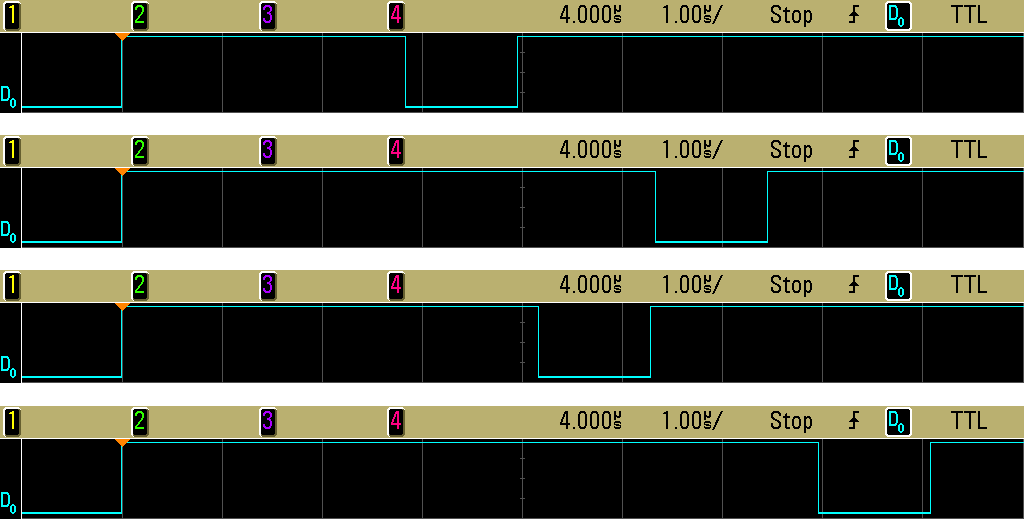
\includegraphics[width=8.5in]{SPI/Figures/spi-waveform_comparison.png}
			\caption{Comparison of arbitration waveforms across all links}
			\label{fig:spi:waveform_comparison}
		\end{centering}
	\end{figure}
\end{landscape}

The code has been tested extensively to ensure correctness. A test has been devised that uses custom code that doesn't contain any non-essential code. While this test is not a real-world scenario, it allows individual sections of code to be tested much more rigorously because the processor won't be spending time running non-essential pieces of code. The test has two nodes continuously transfer known dummy data to each other, and the received flits are checked on the other side for correctness. Each node keeps track of how many flits it sent, how many flits it correctly received, and how many flits were received with errors. This test stresses the arbitration scheme because both nodes are trying to transmit over the same link continuously. The results for each node are shown in Table \ref{tab:spi:endurance_test}. As one can see, the system is perfect at the SPI level. No collisions were tested in this case scenario, unfortunately, because the time window available for a collision to occur is only two to three clock cycles. A few undocumented cases were observed during later testing where collisions were detected and successfully avoided. If a collision is not detected properly, then the flit will simply go missing because the ``receiving'' node is not listening for the exact amount of time that the transmission is occurring. No message garbling occurs.

\begin{table}
	\begin{centering}
		\setlength{\extrarowheight}{1.5pt}
		\caption{SPI Endurance Test}
		\vspace{0.1cm}
		\begin{tabular}{|c|c|c|c|}
			\hline
			\textbf{Node} &	\textbf{Flits Sent} & \textbf{Flits Correctly Received} & \textbf{Flits Incorrectly Received} \\
			\hline
			\hline
	       1 & 500000 & 500000 & 0 \\
	       \hline
	       2 & 500000 & 500000 & 0 \\
	       \hline
		\end{tabular}
		\label{tab:spi:endurance_test}
	\end{centering}
\end{table}
		
\section{Future Work}\label{sec:spi:future_work}

The arbitration scheme discussed here was created rather late in the project. The original scheme called for two arbitration lines that were always owned by a node, regardless of whether or not the port was elevated. This mechanism utilized the STE pin for one of the arbitration lines because it was believed at the time that STE was unnecessary for the prototype hardware, which turned out to be incorrect. A future improvement would be to add the second arbitration pin back to the header link. While the current scheme does guarantee against collisions, it also doubles the amount of time necessary to transmit a flit. The other two-pin arbitration scheme is much faster because it does not need to check the arbitration line twice. Another potential improvement would be to allow link ``ganging,'' i.e. multiple links can be used between two nodes to increase bandwidth. It is also possible to transmit multiple flits together so that a node only  arbitrates once for all of the flits, instead of once per flit. This has the advantage of reducing arbitration overhead, but care would need to be taken to ensure that one node doesn't monopolize the link.

\section{Conclusions}\label{sec:spi:conclusions}

In this chapter, a peer-to-peer variant of SPI was presented that serves as the Physical and Data Link Layers in the prototype toolkit. At the physical layer, an arbitration scheme has been developed that uses an extra GPIO pin for arbitration to prevent collisions, and has been tested thoroughly. At the data link layer, virtual channels have been employed to reduce congestion in the network. Careful attention has been paid to maximizing the effectiveness of buffers on the memory-limited F2808 DSC. This mechanism has shown good robustness and serves as a foundation for the rest of the toolkit.